\section{Introduction}\label{sec:introduction}
% no \IEEEPARstart

Animals use their tails in a variety of ways: to propell through water; to help improve locomotion and balance; and some, like for instance monkeys, have prehensile tails that allow them to grasp trees. Ballance control while running and hopping, even glide control and climbing are some examples of how a tail is helping animals by providing robust locomotion \cite{Thomas:Nature2012}. The use of a tail, or inertial appendages in general, for dynamic stabilization has been reported in dinosaurs, lizards, cats, primates and even humans \cite{ostrom1969osteology,PijnappelsSringer,Walker199841,JusufiIOP2010}. One of the chalanging tasks in biologically inspired robotics is to extract the knowledge from and not simply mimic the nature. Therefore, we seek nature-like solutions on how to use additional appendages to help robot locomotion in the similar way as an animal would do.  

The main reason to use a tail in quadruped robot locomotion is to apply additional forces/torques to stabilize the motion during flight phases in which the robot has no contact with the ground. Uniroo \cite{zeglin1991uniroo} is one of the first robot which uses single degree of freedom(DOF) active tail to maintain constant body pitch while emulate hopping kangaroo. A lizard-inspired active tail stabilization presented in \cite{conf/iros/Chang-SiuLTF11} uses tail on wheeled car which provides robust drive over difficult terrain. The momentum based approach is used only for pitch control. The MIT Cheetah robot \cite{DBLP:conf/iros/BriggsLHK12} uses tail to improve running performance up to 30mph. The authors analize also several others artificial mechanisms which can be used to apply non-contact forces/moments like reaction wheel, reaction mass, thrusters etc. In \cite{PullinICRA12}, Pullin et all compared the use of tail to classical differential drive steering for different surface conditions on a crawling mobile robot OctoRoACH. They showed how a tail could be used when rapid turning or evasive maneuvers are required and on a low friction surface conditions. Learning from Air robots, one can apply the techniques used in \cite{Korpela2013ICRA,Orsag2012JINT} to model the dynamics of inertial appendages and the effect they have on the underlaying robot body.

\begin{figure}
	\centering
	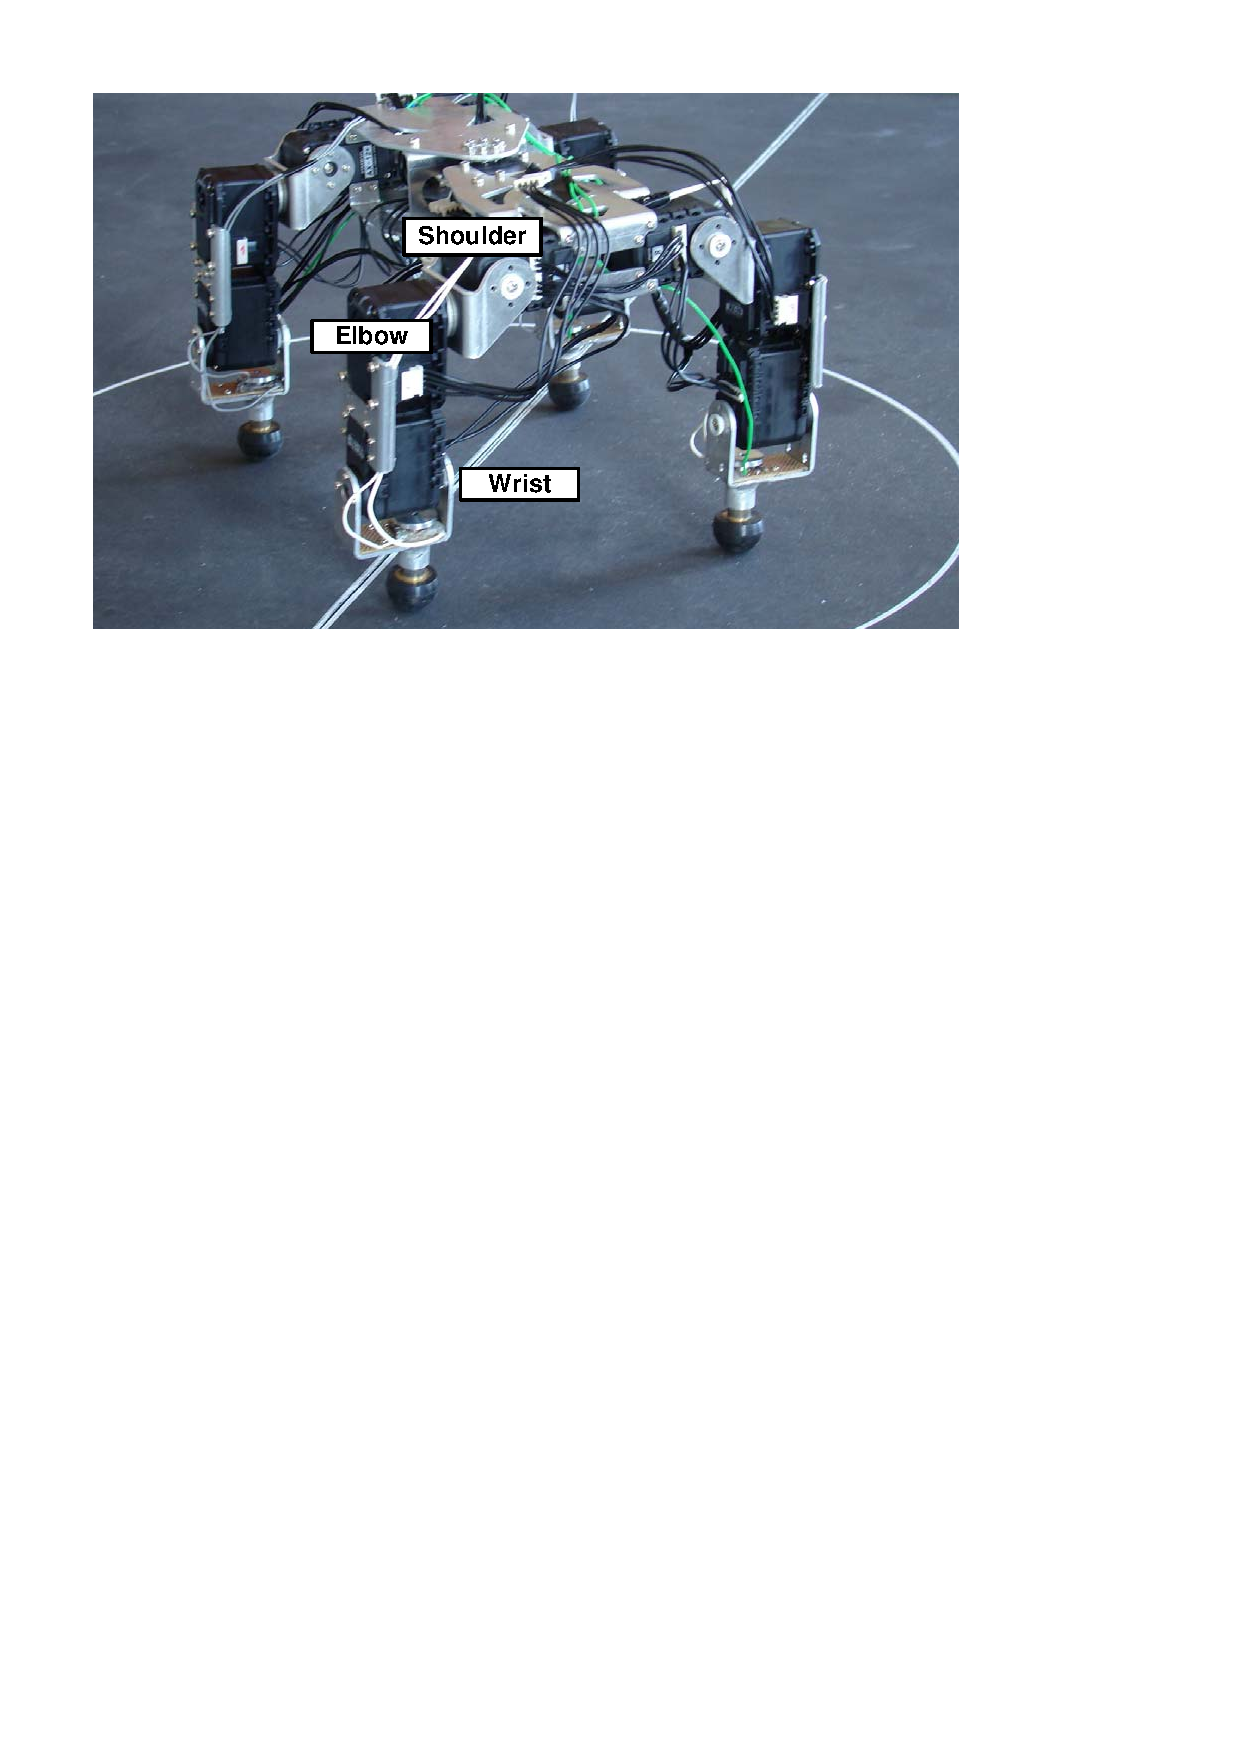
\includegraphics[width=85mm]{./pictures/Dynarobin_introduction_image.pdf}
	\caption{Dynarobin}
	\label{fig:Dynarobin}
\end{figure}

Inspired by the agility of human and animal locomotion, the number of researchers present robot leg design, modeling and control over the last few decades\cite{CambridgeJournals:1345088}. The quadruped locomotion gaits like walking, running, trotting, and bouncing behaves in nature similary as spring-mass models\cite{Blickhan01}. For a single leg, hopping locomotion can be also described by the spring-mass model. In order to obtain active compliant robot leg behaviour, impedance control is used to simulate virtual spring-mass system.\cite{Havoutis01}. Connecting four legs with one central body a complex dynamics problem arises. In order to provide stabile quadrupedal hopping sequence a lot of parameters needs to be observed: mass distribution, active and passive leg stiffness, ground stiffness etc. This paper invetigates how to improove locomotion stability of four spring-mass dynamical system by using the active controlled tail.

In section \ref{sec:Dynarobin} a quadrupedal robot Dynarobin with an impedance control based symplification of its leg dynamics is introduced. Section \ref{sec:MathModel} depicts a complete mathematical model of the robot together with the tail. Building upon the results from \ref{sec:MathModel}, a recursive balancing algorithm is introduced in \ref{sec:Algorithm}. The algorithm is tested in the simulation environment which is described in section \ref{sec:simulation}, along with the simulation results. 





% Some research uses advanced variable stiffnes leg design %\cite{Hurst_2004_4785}\cite{Galloway}\cite{Jun:2009:DSV:1703775.1704089} which allows robot to run over a large variety %of terrains while adjusting their leg stiffness. All this research suggests that quadrupedal robot can be dynamically 5modeled as mass supported on four spring legs as shown in fig. 


